\section{Lösungen zu den Aufgaben aus Vorl 2}
\subsection{Lösung zur 1. Aufgabe: Lineare Regression}
siehe \ref{Vorl2Regressionsaufg1}

zu (a) Stellen Sie das lineare Gleichungssystem auf, das sich durch partielles Ableiten
für das Optimierungsproblem
$$
\min\limits_{a,c,h} \left\{\sum_{j=1}^{J_T} \varepsilon_j^2\right\}
$$
ergibt, mit $J_T = 21$.

Die Modellgleichung lautet
\begin{equation}
z_j \; = \; a \, x_j \, + \, c \, + \, h \, \delta_{j \in C} \; + \; \varepsilon_j
\label{Modellgl1}
\end{equation}
In Vektorschreibweise mit $\boldsymbol x$ und $\boldsymbol z$ als Spaltenvektoren sieht 
dies mit allen in der oben aufgeführten Werten wie folgt aus
$$
\boldsymbol x = \left(
\begin{array}{c}
0\\
0.25\\
0.50\\
\vdots\\
2.25\\
2.75\\
\vdots\\
5.00
\end{array}\right) \qquad
\boldsymbol x_1 = \left(
\begin{array}{c}
1\\
1\\
1\\
\vdots\\
1\\
0\\
\vdots\\
0
\end{array}\right)  \qquad
\boldsymbol x_0 = \left(
\begin{array}{c}
1\\
1\\
1\\
\vdots\\
1\\
1\\
\vdots\\
1
\end{array}\right) \qquad
\boldsymbol z = \left(
\begin{array}{c}
-54.08\\
-55.63\\
-44.65\\
\vdots\\
-60.77\\
36.85\\
\vdots\\
23.19
\end{array}\right)
$$
Für die Realisierung der Kroneckersymbols $\delta_{j \in C}$ wurde
der Spaltenvektor $\boldsymbol x_1$ definiert, der als erste
$J_C = 10$ Vektorkomponenten Einsen enthält und als weitere Vektorkomponenten Nullen.
Der Vektor $\boldsymbol x_0$ besteht nur aus Einsen.

Als nächstes ist es wichtig, die Größen auf dieselbe Dimension zu bringen,
so dass wir eine Steigung berechnen wollen, also rechnen wir die x-Werte auch in Mikrometern
$$
\boldsymbol x_2 \, = \, 1000 \, \boldsymbol x
$$
Somit sieht die Modellgleichung (\ref{Modellgl1}) wie folgt aus
$$
\boldsymbol z \; = \;  c \,  \boldsymbol x_0 \,  + \, h \, \boldsymbol x_1 \, + \, a \, \boldsymbol x_2 \, + \, \boldsymbol \varepsilon
$$
nun schreiben wir alle Spaltenvektoren mit x in eine gemeinsame Matrix, die dann 3 Spalten hat und $J_T = 21$ Zeilen
\begin{equation}
\boldsymbol X \; = \; \left(\boldsymbol x_0 \; \boldsymbol x_1 \; \boldsymbol x_2 \right)
\label{Regressormatrix}
\end{equation}
so dass die Modellgleichung wie folgt aussieht
$$
\boldsymbol \varepsilon  \; = \;  \boldsymbol z \, - \, \boldsymbol X
\left(\begin{array}{c}
c\\
h\\
a
\end{array}\right) .
$$
Wenn man diesen Ansatz in dieser Form hat, kann man einfach Gl.~(\ref{LsgRegressionGlSys}) 
verwenden und alles einsetzten.
Für die Klausur kommt es also nur darauf an, die Regressormatrix $\boldsymbol X$, das ist Gl.~(\ref{Regressormatrix})
aufstellen zu können und Gl.~(\ref{LsgRegressionGlSys}) aus dieser Vorlesung zu kennen:
\begin{equation}
\left( \mathbf{X}^\mathsf{T}  \, \mathbf{X} \right) \left(\begin{array}{c}
c\\
h\\
a
\end{array}\right) \; = \;
 \mathbf{X}^\mathsf{T} \, \mathbf{z} 
\end{equation}
wobei $\boldsymbol X^\mathsf{T}$ die transponierte Matrix ist, die in der ersten Zeile alles Einsen hat, in der
zweiten Zeile an den ersten $J_C = 10$ Spaltenpositionen Einsen und an den letzten 11 Nullen hat und in der dritten
und letzten Zeile die Werte $0.00 ~ 0.25 ~ 0.50 ~ 0.75 \dots ~5.00$ aus der Tabelle hat.
Hier ist dieser Teil der Aufgabenstellung fertig.


zu (b) Schreiben Sie die Gleichung für die Stufenhöhe $d$ als Funktion von $h$ und $a$ auf.
\begin{equation}
d \; = \; \frac{h}{\sqrt{1 + a^2}}
\end{equation}
Wer zuvor die x-Werte in Millimetern gerechnet hat, muss spätestens hier die Steigung
$a$ entsprechend umrechnen und durch $1000$ teilen.

zu (c) Schreiben Sie die Formel für die Varianz der Residuen auf.
$$
\sigma_\varepsilon^2 \; = \; \frac{1}{J_T - 3} \boldsymbol \varepsilon^\mathsf{T} \, \boldsymbol \varepsilon
$$

zu (d) Schreiben Sie die Formel für die Kovarianzmatrix der Modellparameter
$a, c, h$ auf.

Wir verwenden dazu Gl.~(\ref{UnsicherheitRegressparams}) dieser Vorlesung
\begin{equation}
\boldsymbol \Sigma \; = \; \left( \mathbf{X}^\mathsf{T}  \, \mathbf{X} \right)^{-1} \, \sigma_\varepsilon^2
\end{equation}
mit 

zu (e) Verwenden Sie eine Programmierumgebung Ihrer Wahl, Matlab, Octave, Python, R, ...
die Ihnen einen Solver für lineare Gleichungssysteme zur Verfügung stellt, sowie
eine Routine zur Matrixinversion und berechen Sie die Zahlenwerte für die Modellparameter
sowie deren Kovarianzmatrix.

\begin{verbatim}
function Lsg_Uebung_step()
%
% Teil (a)
  x = [0.00  0.25  0.50  0.75  1.00  1.25  1.50 ...
   1.75  2.00  2.25  2.50  2.75  3.00  3.25  3.50 ...
   3.75  4.00  4.25  4.50  4.75  5.00]';
  z = [-54.08 -55.63 -44.65 -51.44 -52.21 -58.01 ...
   -50.76 -56.01 -54.86 -60.77 36.85 38.02 31.71 36.21 ...
   23.39 29.01 30.11 29.35 20.81 33.27 23.19]';
  x2 = 1e3*x;
  J_T = 21;
  J_C = 10;
  x0 = ones(J_T,1);
  x1 = [ones(J_C,1);zeros(J_T-J_C,1)];
  X = [x0 x1 x2];
  XTX = X' * X;
  b = X' * z;
  theta = XTX \ b;
  printf('c = %1.4f um\n', theta(1));
  printf('h = %1.4f um\n', theta(2));
  printf('a = %1.7f um/um\n', theta(3));
\end{verbatim}
\begin{verbatim}
%
% Teil (b)
  d = theta(2) / sqrt(1 + theta(3)^2);
  printf('d = %1.4f um\n', d);
\end{verbatim}
\begin{verbatim}
%
% Teil (c)
  epsilon = z - X * theta;
  var_eps = (epsilon' * epsilon) / (J_T-3);
\end{verbatim}

~\\

\begin{verbatim}
%
% Teil (e)
  Kovarianz = inv(XTX) * var_eps;
  printf(' %e %e %e \n', Kovarianz(1,1), Kovarianz(1,2), Kovarianz(1,3));
  printf(' %e %e %e \n', Kovarianz(2,1), Kovarianz(2,2), Kovarianz(2,3));
  printf(' %e %e %e \n', Kovarianz(3,1), Kovarianz(3,2), Kovarianz(3,3));
\end{verbatim}

Ergebnisse:
\begin{verbatim}
c = 44.5660 um
h = -94.0905 um
a = -0.0038377 um/um
d = -94.0899 um
\end{verbatim}

$\Sigma =$
\begin{verbatim}
2.369818e+01 -1.710178e+01 -5.863466e-03
 -1.710178e+01 1.436549e+01 4.104426e-03
 -5.863466e-03 4.104426e-03 1.563591e-06
\end{verbatim}



\subsection{Lösung zur 2. Aufgabe: Lineare Regression}
siehe \ref{Vorl2Regressionsaufg2}

\textbf{zu Teil (a)} \\
Gesucht: 
\[
Y = \hat\theta_1 \cdot X + \hat \theta_0 
\]
Mittelwert von $X$: $\bar{X} = 3$; Mittelwert von $Y$: $\bar{Y} = 0.64$; \\
Empirische Standardabeichung von $X$: $s_X = 1.5811$; \\
Empirische Standardabeichung von $Y$: $s_Y = 0.1636$; \\
Empirische Kovarianz: $s_{XY} = 0.25$ \\
Schätzwerte $\hat{\theta}_1$ und $\hat{\theta}_0$:
\[
\hat{\theta}_1 = \frac{s_{XY} }{s_X^2 } = 0.100
\]
\[
\hat{\theta}_0 = \bar {Y} - \hat{\theta}_1 \bar {X} = 0.340
\]
Bestimmtheitsmaß:
\[
\rho_{XY}^2 = \frac{s
_{XY}^2 }{s_X^2 \cdot s_Y^2 } = 0.9346
\]
\textbf{zu Teil (b)} \\
Residuen: $\varepsilon_j = Y_j -(\hat\theta _0 + \hat\theta _1 \cdot X_j)$
mit $j=1,\ldots ,5$
 \[\varepsilon_1 = -0.0400; \;\; \varepsilon_2 =  0.0100;\;\;
 \varepsilon_3= 0.0600;\;\; \varepsilon_4 =0.0100;\;\;
  \varepsilon_5 = -0.0400
 \]
Qualitätsmaß:
\[
Q(\hat\theta _0,\hat\theta _1) = \sum\limits_{j = 1}^J {\varepsilon_j ^2 } 
= 0.0070
\]
Varianz der Residuen:
\[
s^2(\hat{\theta}_0 ,\hat{\theta}_1 ) = \frac{Q(\hat{\theta}_0 ,
	\hat{\theta}_1 )}{J - 2} = 0.0023 \quad \text{bzw.} \quad
     s(\hat{\theta}_0 ,\hat{\theta}_1 ) = 0.048 
\]
\textbf{zu Teil (c)} \\
Die Standardabweichung für $X$ berechnet sich zu $s_X = 1.5811$.

Für die Varianz des y-Abschnitt $\hat\theta_0$ ergibt sich: 
\begin{eqnarray}
\hat\sigma_{\theta_0}^2 &=& s^2(\hat{\theta}_0 ,\hat{\theta}_1 )
\left[\frac{1}{J} + \frac{\bar{X}^2}{(J-1)s_x^2 } \right]
\nonumber \\ 
&=& 
0.0023
\left[\frac{1}{5} + \frac{3^2}{(5-1)\cdot 1.5811^2 } \right]
 \nonumber\\ 
&=& 0.00253 \nonumber
\end{eqnarray}
Damit ergibt sich die Standardabweichung für $\hat\theta_0$:
\[
s_{\hat\theta_0} = \sqrt{\hat\sigma_{\theta_0}^2} = 0.0503
\]
Für die Varianz der Steigung $\hat\theta_1$ ergibt sich: 

\begin{eqnarray}
\hat\sigma^2_{\theta_1} &=& \frac{ \hat s^2(\hat{\theta}_0 ,\hat{\theta}_1 )}
{s^2_X \cdot (J- 1) }
\nonumber \\
&=& \frac{ 0.0023}
{1.5811^2 \cdot (5- 1) } \nonumber \\
&=& 0.00023
\end{eqnarray}

Damit ergibt sich die Standardabweichung für $\hat\theta_1$
\[
s_{\hat\theta_1} = \sqrt{\hat\sigma_{\theta_1}^2} = 0.01517
\]

\newpage
\textbf{Anmerkung: Lösung mit Matlab/Octave} 
Bei Matlab gibt es den Befehl \glqq polyfit\grqq ~mit dem Polynomfits durchgeführt werden können. Matlab liefert hier dasselbe Ergebnis, auch für die Vertrauensbereiche, das Qualitätsmaß $Q$ (engl. SSE: Sum sqared error) oder das Bestimmheitsmaß $\rho^2_{XY}$ (R-square), siehe Abb.\ref{fig:MatlabPolyfit}:
\begin{figure}[!htp]
	\begin{center}
		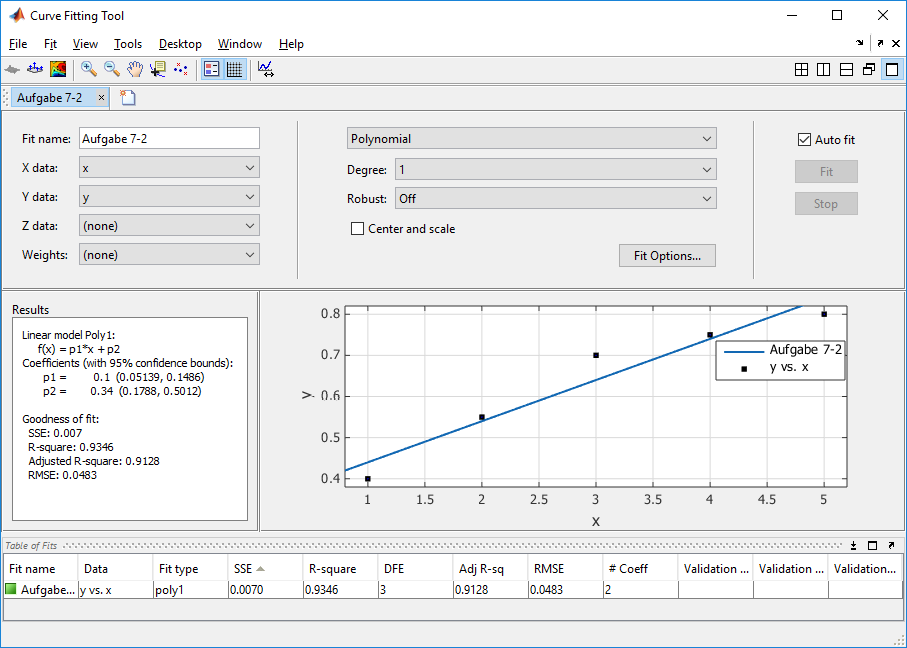
\includegraphics[width=160mm]{02_vorlesung/media/Matlab_CFTool.png}
		\caption{Lösung der Aufgabe mit dem polyfit Befehl von Matlab/Octave. 
		Es wird hier u.~a. der 95\%ige Vertrauensbereich berechnet und
		angezeigt (siehe Mitte links in der Abbildung).}
		\label{fig:MatlabPolyfit}
	\end{center}
\end{figure}

\textbf{Hinweis: Vertrauensbereich} \\
In einer der nächsten Vorlesungen werden wir sehen wie man Vertrauensbereiche 
mit Hilfe der Varianzen bzw. Standardabweichungen berechnet. Dazu benötigt man 
noch die t-Verteilung. Da man hier 5 Messpunkte und 2 Modellparameter hat,
wird die t-Verteilung mit dem Freiheitsgrad 5-2 = 3 benötigt. 
95\%iger Vertrauensbereich für $\hat\theta_1$ mit $t_3 = 3.182$: 
\[
\varepsilon _{\hat{\theta}_1} = t_3 \cdot \hat\sigma_{\theta_1} = \frac{t_3 \cdot s(\hat{\theta}_0 ,
	\hat{\theta}_1 )}{s_X \cdot \sqrt {J
		- 1} } = 0.0486
\]
95\%iger Vertrauensbereich für $\hat\theta_0$ errechnet sich durch:
\[
\varepsilon _{\hat{\theta}_0} = t_3 \cdot \hat\sigma_{\theta_0} = t_3 \cdot s(\hat{\theta}_0 ,\hat{\theta}_1 ) \cdot \sqrt {\frac{1}{J} + \frac{\bar {X}^2}{(J - 1) s_X^2 }} = 0.1612
\]
\textbf{Ergebnis:} \\ 
Der 95\% Vertrauensbereich des Schätzwertes $\hat\theta_1$ ist somit gegeben durch:
\begin{equation}
\hat\theta_1 = 0.1000 \pm 0.0486 \quad \text{bzw.} \quad [0.0514;0.1486]
\end{equation}
Der 95\% Vertrauensbereich des Schätzwertes $\hat\theta_0$ ist somit gegeben durch: 
\begin{equation}
\hat\theta_1 = 0.3400 \pm 0.1612 \quad \text{bzw.} \quad [0.1788;0.5012]
\end{equation}


\begin{comment}
95\%iger Vertrauensbereich für $\hat\theta_1$ mit $t_3 = 3.182$ und 
Standardabweichung von $s_X = 1.5811$
\[
\varepsilon _{\hat{\theta}_1} = \frac{t_3 \cdot s(\hat{\theta}_0 ,
\hat{\theta}_1 )}{s_X \cdot \sqrt {J
- 1} } = 0.0486
\]
95\%iger Vertrauensbereich für $\hat\theta_0$ errechnet sich durch:
\[
\varepsilon _{\hat{\theta}_0} = t_3 \cdot s(\hat{\theta}_0 ,\hat{\theta}_1 ) \cdot \sqrt {\frac{1}{J} + \frac{\bar {X}^2}{(J - 1) s_X^2 }} = 0.1612
\]
\textbf{Ergebnis:} \\ 
Der 95\% Vertrauensbereich des Schätzwertes $\hat\theta_1$ ist somit gegeben durch:
\begin{equation}
\hat\theta_1 = 0.1000 \pm 0.0486 \quad \text{bzw.} \quad [0.0514;0.1486]
\end{equation}
Der 95\% Vertrauensbereich des Schätzwertes $\hat\theta_0$ ist somit gegeben durch: 
\begin{equation}
\hat\theta_1 = 0.3400 \pm 0.1612 \quad \text{bzw.} \quad [0.1788;0.5012]
\end{equation}
\end{comment}


\pagebreak

Für die Unermüdlichen, die lieber in C programmieren, hier die Routine zum Lösen
des linearen Gleichungssystems, haben wir eine Routine zum Lösen von linearen
Gleichungssystemen aus den Numerical Recipes abgedruckt:

B. P. Flannery, W. H. Press, S. A. Teukolsky, W. T. Vetterling. \textsl{Numerical Recipes
in C}. Cambridge University Press, 2.~Auflage (1992-2002)

Wichtig, diese Routine überschreibt den Vektor mit der Inhomogenität des Gleichungssystems
mit der Lösung, also den gewünschten Modellparametern und 
die Matrix \texttt{a} mit den Summen aus den Regressoren mit deren Inversen
\texttt{a}$^{-1}$, die Sie dann für die Kovarianz der Modellparameter brauchen.

\begin{verbatim}
void gaussjordan(double **a, int n, double **b, int m)
/*
* Linear equation solution by Gauss-Jordan elimination, equation (2.1.1) in
* Numerical Recipes.
* a[0..n-1][0..n-1] is the input matrix. b[0..m-1][0..n-1] is input
* containing the m right-hand side vectors.
* For most applications we have m = 1
* On output, a is replaced by its matrix inverse,
* and b is replaced by the corresponding set of solution vectors.
*/
int *indxc,*indxr,*ipiv;
int i,icol,irow,j,k,l,ll;
double big,tmp,pivinv;

// The integer arrays ipiv, indxr, and indxc are
// used for bookkeeping on the pivoting.
indxc = (int*)calloc( n, sizeof(int));
indxr = (int*)calloc( n, sizeof(int));

ipiv = (int*)calloc( n, sizeof(int));

/*	for (j=1;j<=n;j++) ipiv[j]=0;*/
/*	for (j=1;j<=n;j++) ipiv[j]=0;*/
/* calloc initializes to zero:
Allocates a block of memory for an array of num elements,
each of them size bytes long, and initializes all its bits to zero.
*/

/*
* This is the main loop over the columns to be reduced.
*/
for (i=0; i<n; i++) {
big=0.0;

// This is the outer loop of the search for a pivot element.
for (j=0; j<n; j++)
if (ipiv[j] != 1)
for (k=0; k<n; k++) {
if (ipiv[k] == 0) {
if (fabs(a[k][j]) >= big) {
big=fabs(a[k][j]);
irow=j;
icol=k;
}
}
}
++(ipiv[icol]);

/*
* We now have the pivot element, so we interchange rows, if needed,
* to put the pivot element on the diagonal. The columns are not
* physically interchanged, only relabeled:
* indxc[i], the column of the ith pivot element,
*           is the ith column that is reduced, while
* indxr[i] is the row in which that pivot element was originally located.
*          If indxr[i] !=
* indxc[i] there is an implied column interchange.
* With this form of bookkeeping, the solution b-s will end up in the
* correct order, and the inverse matrix will be scrambled by columns.
*/

if (irow != icol) {
for (l=0; l<n; l++) SWAP(a[l][irow],a[l][icol])
for (l=0; l<m; l++) SWAP(b[l][irow],b[l][icol])
}

/*
* We are now ready to divide the pivot row by the
* pivot element, located at irow and icol.
*/

indxr[i]=irow;
indxc[i]=icol;
if (a[icol][icol] == 0.0) printf("gaussj: Singular Matrix\n");
pivinv=1.0/a[icol][icol];
a[icol][icol]=1.0;
for (l=0; l<n; l++) a[l][icol] *= pivinv;
for (l=0; l<m; l++) b[l][icol] *= pivinv;

/*
* Next, we reduce the rows
* except, if (ll != icol), for the pivot one, of course.
*/
for (ll=0; ll<n; ll++)
if (ll != icol) {
tmp=a[icol][ll];
a[icol][ll]=0.0;
for (l=0; l<n; l++) a[l][ll] -= a[l][icol]*tmp;
for (l=0; l<m; l++) b[l][ll] -= b[l][icol]*tmp;
}
}
/*
* This is the end of the main loop over columns of the reduction.
*/

/*
* It only remains to unscramble the solution in view of the column interchanges.
* We do this by interchanging pairs ofcolumns in the reverse order
* that the permutation was built up.
*/
for (l=n-1; l>=0;l--) {
if (indxr[l] != indxc[l])
for (k=0; k<n; k++) SWAP(a[indxr[l]][k],a[indxc[l]][k]);
}
// And we are done.
free(ipiv);
free(indxr);
free(indxc);
}
\end{verbatim}


